\documentclass[11pt]{article}
\usepackage{vmargin}
\setpapersize{A4}
\setmargins{15mm}{10mm}{180mm}{252 mm}%
             {16mm}{2mm}{0pt}{10mm}
\usepackage[french]{babel}

\usepackage{lmodern} 
\usepackage[T1]{fontenc}
\usepackage{fouriernc}
\usepackage{eurosym} % pour le symbole euro
\usepackage{graphicx} 
\usepackage{array} 
\usepackage{tabularx}
\usepackage{variations}
\usepackage{amsmath} 
\usepackage{amssymb}
\usepackage{epic} % pour le dessin avec l'environnment picture
\usepackage{rotating}
\usepackage[autolanguage]{numprint}
\usepackage[tikz]{bclogo} 

\usepackage{circuitikz} % circuit electriques

\setlength{\unitlength}{1 mm}
\usepackage{xy} % pour la réalisation de dessin, graphique, diagramme
\xyoption{all}

\newcommand{\cadreblanc}[1]{%
\medskip\framebox[\linewidth][c]{%
\rule{0mm}{#1mm}}\par
\medskip}


\def\labelenumii{\theenumi.~\theenumii.}
\def\theenumii{\arabic{enumii}}


\presetkeys{bclogo}{logo=\bcquestion,couleur=gray!10,barre=snake,arrondi = 0.1}{}

%%%%%%%%%%%%%%%%%%%%%%%%%%%%%%%%%%%%%%%%%%%%%%%%%%%%%%%%%%
%
% Définition des sections et sous-sections
%
%%%%%%%%%%%%%%%%%%%%%%%%%%%%%%%%%%%%%%%%%%%%%%%%%%%%%%%%%%


\renewcommand{\thesection}{{\arabic{section}.}}

\addto\captionsfrench{\def\tablename{Document}}
\usepackage{setspace}
\usepackage{multicol}
\usepackage{multirow}
\usepackage{fancyhdr}
\usepackage{graphpap}

%%%%%%%%%%%%%%%%%%%%%%%%%%%%%%%%%%%%%%%%%%%%%%%%%%%%%%%%%%
%
% Définition de nouveaux types de colonne
%
%%%%%%%%%%%%%%%%%%%%%%%%%%%%%%%%%%%%%%%%%%%%%%%%%%%%%%%%%%

\newcolumntype{C}{>{\centering\arraybackslash}X}
\newcolumntype{L}{>{\raggedright\arraybackslash}X}
\newcolumntype{R}{>{\raggedleft\arraybackslash}X}


\renewcommand{\footrulewidth}{0.4pt}
\usepackage{lastpage} 

\newcommand{\appel}{\raisebox{-2ex}{
\includegraphics[width=1cm]{images/appel.jpg}}\quad}



%%%%%%%%%%%%%%%%%%%%%%%%%%%%%%%%%%%%%%%%%%%%%%%%%%%%%%%%%%
%                                                        %
%              Evaluation par compétences                %
%                                                        %
%%%%%%%%%%%%%%%%%%%%%%%%%%%%%%%%%%%%%%%%%%%%%%%%%%%%%%%%%%



\newcommand\SA{\marginpar{\scalebox{.8}{\framebox[1.6ex]{\rule{0ex}{1.6ex}\raisebox{.75ex}{\rule{1.6ex}{.5pt}}}\hspace{-.3pt}\framebox[3.2ex]{S}}}}
\newcommand\A{\marginpar{\scalebox{.8}{\framebox[1.6ex]{\rule{0ex}{1.6ex}\raisebox{.75ex}{\rule{1.6ex}{.5pt}}}\hspace{-.3pt}\framebox[3.2ex]{A}}}}
\newcommand\R{\marginpar{\scalebox{.8}{\framebox[1.6ex]{\rule{0ex}{1.6ex}\raisebox{.75ex}{\rule{1.6ex}{.5pt}}}\hspace{-.3pt}\framebox[3.2ex]{R}}}}
\newcommand\V{\marginpar{\scalebox{.8}{\framebox[1.6ex]{\rule{0ex}{1.6ex}\raisebox{.75ex}{\rule{1.6ex}{.5pt}}}\hspace{-.3pt}\framebox[3.2ex]{V}}}}
\newcommand\C{\marginpar{\scalebox{.8}{\framebox[1.6ex]{\rule{0ex}{1.6ex}\raisebox{.75ex}{\rule{1.6ex}{.5pt}}}\hspace{-.3pt}\framebox[3.2ex]{C}}}}


%%%%%%%%%%%%%%%%%%%%%%%%%%%%%%%%%%%%%%%%%%%%%%%%%%%%%%%%%%
%                                                        %
% Définitions de l'année, la spécialité, du diplome ...  %
%                                                        %
%%%%%%%%%%%%%%%%%%%%%%%%%%%%%%%%%%%%%%%%%%%%%%%%%%%%%%%%%%


\newcommand{\specialite}{Systèmes Numériques}
\newcommand{\annee}{2023-2024}
\newcommand{\diplome}{Baccalauréat Professionnel}
\newcommand{\etablissement}{LP Denis Diderot}
\newcommand{\classe}{TSN1}
\newcommand{\datedeval}{\today}
\newcommand{\matiere}{Sciences Physiques et chimiques }

\newcommand{\sequence}{2/2}


%%%%%%%%%%%%%%%%%%%%%%%%%%%%%%%%%%%%%%%%%%%%%%%%%%%%%%%%%%
%                                                        %
% Définitions des capacités, connaissances et attitudes. %
%                                                        %
%%%%%%%%%%%%%%%%%%%%%%%%%%%%%%%%%%%%%%%%%%%%%%%%%%%%%%%%%%


\newcommand{\theme}{
Caractériser la propagation d'un signal sonore.}


\newcommand{\capacites}{
  \begin{minipage}[c]{12.5cm}
    \begin{itemize}
      \item \rule{0ex}{2.5ex}Exploiter la relation liant la vitesse de propagation, la longueur d'onde et la fréquence d'une onde sonore.
      \item  Déterminer expérimentalement la vitesse de propagation d'un son dans l'air ou dans l'eau. \rule[-1.5ex]{0ex}{3ex} 
      \end{itemize}
    \end{minipage}
  }


\newcommand{\connaissances}{
  \begin{minipage}[c]{12.5cm}
    \begin{itemize}
    \item \rule{0ex}{2.5ex}Savoir que la propagation d?un son nécessite un milieu matériel.
    \item Savoir que la vitesse du son dépend du milieu de propagation.  
    \item Connaître la relation qui lie la longueur d'onde, la vitesse de propagation et la période d'une onde sonore $\lambda = c \times T$  
    \item Connaître les ordres de grandeur des vitesses de
propagation du son dans l'air et dans l'eau.\rule[-1.5ex]{0ex}{3ex}
    \end{itemize}
    \end{minipage}
  }

\newcommand{\attitudes}{
  \begin{minipage}[c]{12.5cm}
    \begin{itemize}
    \item \rule{0ex}{2.5ex}Le sens de l'observation.
    \item L'ouverture à la communication, au dialogue et au débat argumenté.
    \item La rigueur et la précision
    \item Le respect des règles élémentaires de sécurité. 
    \item \rule[-1.5ex]{0ex}{3ex}Le gout de chercher et de raisonner.
    \end{itemize}
  \end{minipage}
}




%%%%%%%%%%%%%%%%%%%%%%%%%%%%%%%%%%%%%%%%%%%%%%%%%%%%%%%%%%
%                                                        %
%                   Début du document                    %
%                                                        %
%%%%%%%%%%%%%%%%%%%%%%%%%%%%%%%%%%%%%%%%%%%%%%%%%%%%%%%%%%





%%%%%%%%%%%%%%%%%%%%%%%%%%%%%%%%%%%%%%%%%%%%%%%%%%%%%%%%%%
%                                                        %
%                     Page de garde                      %
%                                                        %
%%%%%%%%%%%%%%%%%%%%%%%%%%%%%%%%%%%%%%%%%%%%%%%%%%%%%%%%%%



\begin{document}
\pagestyle{fancy}
\lfoot{Alexis Ruiz}
\cfoot{\thepage/3}
\rfoot{\datedeval}

\thispagestyle{empty}
\Large 
\noindent\begin{tabularx}{1\linewidth}[c]{|c|c|c|C|C|}
  \hline
  \multirow{2}{*}{
  \begin{minipage}[c]{3cm}
    
\includegraphics[width=30mm]{images/aca-besancon.png}
  \end{minipage}}   &
 \multicolumn{4}{c|}{
 \begin{minipage}[c]{12cm}
      \begin{center}
         \rule[-1.5ex]{0ex}{5ex}BACCALAURÉAT PROFESSIONNEL\\
         \rule[-2ex]{0ex}{4ex} \specialite 
      \end{center}    \end{minipage}}\\
  \cline{2-5}
  & \multicolumn{3}{c|}{\rule[-2ex]{0ex}{5.5ex}Épreuve E1- Sciences Physiques et chimiques } & Coef. 2\\
  \hline
  \multirow{2}{*}{
  \begin{minipage}[c]{3cm}
    \begin{center}
      Contrôle en \\ Cours de\\ Formation
    \end{center}      
    \end{minipage}}
    &
  \multirow{2}{*}{
    \raisebox{-2ex}{\begin{minipage}[c]{6.3cm}
      \begin{center}
        Situation d'évaluation de\\ \matiere
     \end{center}  
    \end{minipage}}}
    &
  \multirow{2}{*}{
    \begin{minipage}[c]{2.2cm}
      \begin{center}
        Année\\ scolaire\\ \annee
  \end{center}  
    \end{minipage}}
    &
    \rule[-1ex]{0ex}{4ex}Séquence &
    Durée\\
    \cline{4-5}
    &&&
    \rule[-1.5ex]{0ex}{5ex}\sequence
    & 
    45~min
\\
\hline
\end{tabularx}

\bigskip

\noindent\fbox{
  \begin{minipage}[c]{.97\linewidth}
    \centerline{\rule[-.8ex]{0ex}{3.5ex}FICHE D'INFORMATION DU CANDIDAT}
  \end{minipage}
}

\bigskip


\normalsize

\noindent\begin{tabularx}{1\linewidth}{|p{11cm}C|}
  \hline
  \rule{0ex}{3ex}Établissement~:~\textbf{{\etablissement}} & Classe~:~\textbf{\classe}\\
 \rule[-1ex]{0ex}{4ex} NOM et Prénom du CANDIDAT : \ \dotfill & Date de l'évaluation~:~\textbf{\datedeval}\\
 \hline
\end{tabularx}
\bigskip

\noindent{\Large Thème~: \theme}\\

\noindent{\Large Module(s) évalué(s)~: }

\begin{center}
  Capacités, connaissances et attitudes du référentiel évaluées\\
  \begin{tabularx}{16cm}{|C|l|}
    \hline
    \textbf{Capacités} &
    \capacites\\
    \hline 
    \textbf{Connaissances} &
    \connaissances    \\
    \hline
    \textbf{Attitudes}  &
    \attitudes\\
    \hline
  \end{tabularx}
\end{center}

\noindent\fbox{\begin{minipage}[c]{.97\linewidth}
    \begin{description}
  \item[$\vartriangleright$] La clarté des raisonnements et la qualité de la rédaction
    interviendront dans l'appréciation des copies.
  \item[$\vartriangleright$] L'emploi des calculatrices est autorisé, dans les conditions
    prévues par la réglementation en vigueur.
  \end{description}
\end{minipage}}

\bigskip


L'évaluation est notée sur 10 : 7 points pour la mobilisation des
connaissances et des compétences pour résoudre des problèmes et 3
points pour l'activité d'expérimentation.

\begin{center}
  \begin{tabularx}{1\linewidth}{|L|c|}
  \hline
  \textbf{\rule{0ex}{3ex}Le candidat atteste avoir été informé de la date et des objectifs
    de l'évaluation le \makebox[4cm]{\rule{0ex}{3ex}\dotfill}} & \textbf{\rule[-6ex]{0ex}{3ex}\underline{Émargement}}\\
   \hline
\end{tabularx}
\end{center}


%%%%%%%%%%%%%%%%%%%%%%%%%%%%%%%%%%%%%%%%%%%%%%%%%%%%%%%%%%
%                                                        %
%                   fin page de garde                    %
%                                                        %
%%%%%%%%%%%%%%%%%%%%%%%%%%%%%%%%%%%%%%%%%%%%%%%%%%%%%%%%%%


\newpage

\lhead{\textbf{\matiere}}
\rhead{Année scolaire \annee}
\setcounter{page}{1}
\large

\noindent\begin{tabularx}{1\linewidth}[c]{|c|c|C|C|}
  \hline
  \multirow{2}{*}{\Large
    \begin{minipage}[c]{4cm}
      \begin{center}
        Contrôle en Cours\\ de Formation
    \end{center}      
  \end{minipage}}
    &
    \multirow{2}{*}{
      \begin{minipage}[c]{7.2cm}
        \begin{center}
          Situation de Sciences Physiques et chimiques
        \end{center}  
    \end{minipage}}
  &
  \rule[-1ex]{0ex}{4ex}Séquence &
  Durée\\
  \cline{3-4}
  &&
    \rule[-1.5ex]{0ex}{5ex}2/2
    & 
    45~min\\
\hline
\end{tabularx}
\medskip


\noindent\fbox{
  \Large\begin{minipage}[c]{.97\linewidth}
    \centerline{\rule[-.8ex]{0ex}{3.5ex}SUJET DESTINÉ AU CANDIDAT}
  \end{minipage}
}

\medskip

\noindent\begin{tabularx}{1\linewidth}{|p{10cm}L|}
  \hline
  \rule{0ex}{3ex}Établissement:~\textbf{{\etablissement}} & Classe~:~\textbf{\classe}\\
 \rule[-1ex]{0ex}{4ex} NOM et Prénom : \ \dotfill & Date de l'évaluation : \textbf{\datedeval}\\
 \hline
\end{tabularx}

\medskip


\noindent\begin{tabularx}{1\linewidth}{|c|L|}
  \hline
\multirow{2}{1.3cm}{\ \appel} & \textbf{\rule[-.8ex]{0ex}{3.5ex}L'examinateur intervient à la demande du
candidat ou quand il le juge utile.}\\
\cline{2-2} 
&\textbf{\rule[-.8ex]{0ex}{3.5ex}Dans la suite du document, ce symbole signifie <<Appeler
  l'examinateur>>.}\\
 \hline
\end{tabularx}

\bigskip

\noindent
\normalsize
\setstretch{1.2}

\parindent 0cm


\noindent
  \setlength{\arraycolsep}{2pt}
  \begin{bclogo}[logo=\bcinfo]
{Situation~:}
\begin{center}
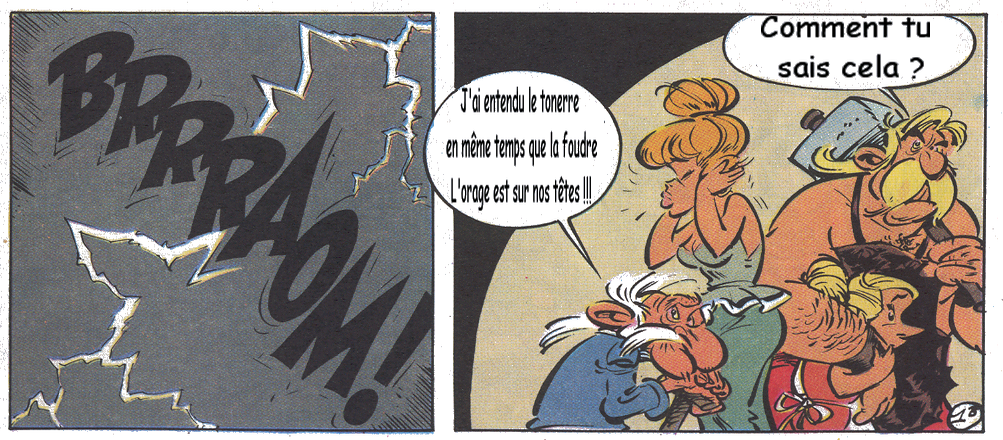
\includegraphics[scale=0.4]{images/asterix.png} 
\end{center}
\end{bclogo}


\vfill

\begin{bclogo}{~Problématique :}
    \begin{center}
    \textbf{Pourquoi voit-on toujours l'éclair avant d'entendre le tonnerre ?}
    \end{center}
\end{bclogo}
\vfill

\textbf{1. Compréhension et analyse de la situation / formulation d'une hypothèse.\\}
\textbf{1.1. Proposer une explication à ce phénomène : \\[15pt]}
\begin{minipage}[c]{.91\linewidth}
    .\dotfill\\
    
    .\dotfill\\
  \end{minipage}\SA\A
\vfill

\textbf{1.2. Proposer une expérience permettant de mesurer la vitesse du son : \\[10pt]}
\begin{minipage}[c]{.91\linewidth}
\cadreblanc{40}
  \end{minipage}\A\C



\newpage
    
\textbf{2. Expérimentation / modélisation de la situation}\\
Afin de déterminer la vitesse du son dans l'air, on se propose de mesurer la longueur d'onde d'un signal sonore. \\

\textbf{2.1. Réaliser le montage suivant et effectuer les réglages demandés :  }\\
\begin{center}
\fbox{\textbf{Ne pas mettre sous tension}}
\end{center}
\begin{center}
\fbox{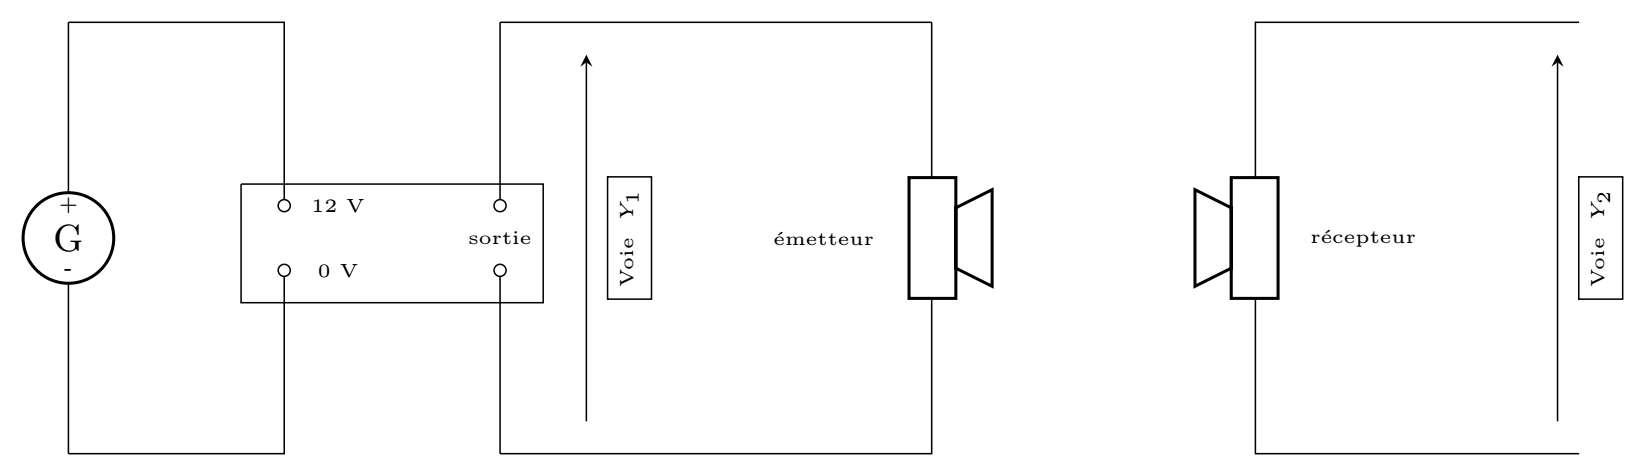
\includegraphics[scale=0.45]{images/montageUS.png} }
\end{center}
\SA\R

  \vfill
\begin{center}


\begin{itemize}

\leftskip=2.5cm

\item[$\square$] L'émetteur et le récepteur sont orientés l'un vers l'autre suivant un axe horizontal. \\
\item[$\square$] Le récepteur est placé à la verticale du zéro de la graduation de la règle.\\
\item[$\square$] Régler l'oscilloscope : 	base temps $5 \mu s$ ; base tension : la plus adaptée.

\item[$\times$] Ne pas toucher aux réglages du convertisseur\\

\leftskip=0cm

\end{itemize}



\end{center}

  \vfill
  

\noindent\begin{tabularx}{0.99\linewidth}{|c|L|}
  \hline
\multirow{2}{1.3cm}{\ \appel} & \textbf{\rule[-.8ex]{0ex}{3.5ex}Appel n$^\circ$ 1.}\\

&{\rule[-.8ex]{0ex}{3.5ex}Faire vérifier le montage et proposer une explication orale à ce phénomène .}\\
 \hline
\end{tabularx}
  \C
\vfill

\textbf{2.2. Comparer les valeurs des périodes des tensions de l'émetteur ($Y_1$) et du récepteur ($Y_2$). }\\[15pt]

\begin{minipage}[c]{.91\linewidth}
    .\dotfill\\
    
    .\dotfill\\
  \end{minipage}\V
  
  \vfill
  
  
\textbf{2.3. Calculer, en s, la période des signaux.}\\[15pt]
\begin{minipage}[c]{.99\linewidth}
    \cadreblanc{25}
  \end{minipage}\SA\R
  
  \vfill
  \noindent\begin{tabularx}{0.99\linewidth}{|c|L|}
  \hline
\multirow{2}{1.3cm}{\ \appel} & \textbf{\rule[-.8ex]{0ex}{3.5ex}Appel n$^\circ$ 2.}\\

&{\rule[-.8ex]{0ex}{3.5ex}Proposer oralement une méthode permettant d'obtenir avec une précision importante la valeur, en m, de la longueur d'onde $\lambda$.}\\
 \hline
\end{tabularx}
\A\C
  \vfill




\newpage

\textbf{2.4. Effectuer la manipulation proposée et noter, en m, la valeur de la longueur d'onde $\lambda$. }\\[25pt]
\begin{minipage}[c]{.91\linewidth}
    .\dotfill\\
  \end{minipage}\R
  
  \vfill
  
\textbf{3. Exploitation, conclusion}\\[5pt]
\textbf{3.1. En vous aidant du formulaire ci-dessous, calculer la vitesse v, en m/s, de l'onde sonore. }\\

\begin{bclogo}[logo=\bcinfo,arrondi=.1,couleur=gray!10,barre=snake,ombre = true, epOmbre = 0.15, couleurOmbre = black!30]{~Formulaire}
    \begin{minipage}[c]{7.4cm}
        \begin{center}
        $\lambda= v \times T$
        \end{center}
    \end{minipage}
    \hfill \vrule \hfill
    \begin{minipage}[c]{9.1cm}
      \textbf{avec } 
      \begin{itemize}
      \item[$\bullet$] $\lambda$ la longueur d'onde en $m$.
      \item[$\bullet$] $v$ la vitesse de l'onde sonore en $m/s$ 
      \item[$\bullet$] $T$ la période en $s$
      \end{itemize}
    \end{minipage}
\end{bclogo}

\begin{minipage}[c]{.99\linewidth}
    \cadreblanc{25}
  \end{minipage}\R


\vfill

\textbf{3.2. Cette valeur est-elle en accord avec celle déterminée en cours ?  }\\[25pt]
\begin{minipage}[c]{.91\linewidth}
    .\dotfill\\
  \end{minipage}\V
  
\vfill

\textbf{3.3. En vous aidant du texte ci-dessous, déterminer, en Mach, la vitesse de la lumière\\
 ~~~~~~($v = 300 000 km/s$). }\\

\begin{bclogo}[logo=\bcinfo,arrondi=.1,couleur=gray!10,barre=snake,ombre = true, epOmbre = 0.15, couleurOmbre = black!30]{}
lorsqu'on dit qu'un avion passe le mur du son, c'est qu'il atteint et dépasse la vitesse du son dans l'air. L'appareil vole au moins à 340m/s, équivalent à 1.224 km/h. On dit alors qu'il atteint Mach 1 (les Mach indiquent la vitesse d'un corps par rapport à la vitesse du son : Mach 1 = une fois cette vitesse ; Mach 2 = deux fois). 
\end{bclogo}
\SA\R\C
\cadreblanc {25}

\vline 

\begin{bclogo}[logo=\bcinfo,arrondi=.1,couleur=gray!10,barre=snake,ombre = true, epOmbre = 0.15, couleurOmbre = black!30]{Où en sommes nous ? }
La sonde Packer  en frôlant le soleil ce 29 avril 2022 à 532 000 km/h est devenue l'objet est le plus rapide jamais conçu par l'humanité. Fabriquée par la NASA, elle peut ainsi parcourir plus de 140 kilomètres en une seconde. À cette vitesse, elle pourrait rejoindre la Lune depuis la Terre en seulement 43 minutes (source  Futura Sciences).
\end{bclogo}

\vline 

\newpage

%%%%%%%%%%%%%%%%%%%%%%%%%%%%%%%%%%%%%%%%%%%%%%
%%%%%%%%%%%%%%%%%%%%%%%%%%%%%%%%%%%%%%%%%%%%%%
%%                                          %%
%%          Fiche d'évaluation              %%
%%                                          %%
%%%%%%%%%%%%%%%%%%%%%%%%%%%%%%%%%%%%%%%%%%%%%%
%%%%%%%%%%%%%%%%%%%%%%%%%%%%%%%%%%%%%%%%%%%%%%

\small

\thispagestyle{empty}
\setstretch{1}

\noindent\begin{tabularx}{1\linewidth}[c]{|L|l|l|}
  \hline
  \multicolumn{3}{|c|}{\large
    \begin{minipage}[c]{.7\linewidth}
      \begin{center}
        \bfseries \rule{0ex}{3ex}GRILLE NATIONALE D'ÉVALUATION

        EN MATHÉMATIQUES ET EN

        SCIENCES PHYSIQUES ET CHIMIQUES\rule[-1ex]{0ex}{3ex}
      \end{center}
    \end{minipage}
}\\
  \hline
  \rule[-1ex]{0ex}{4ex} Nom : & \rule{.3cm}{0cm}Diplôme
  préparé : \diplome\rule{.3cm}{0cm} &  Séquence
  d'évaluation\footnote{Chaque séquence propose la résolution de 
    problèmes issus du domaine professionnel ou de la vie courante. En
    mathématiques, elle comporte un ou deux exercices ; la résolution
    de l'un d'eux nécessite la mise en \oe{}uvre de capacités
    expérimentales.} \no\sequence \\
 \hline\end{tabularx}\\[.3cm]


\textbf{1.  Liste des capacités, connaissances et attitudes évaluées} 
\begin{center}
  \begin{tabularx}{1\linewidth}{|C|l|}
    \hline
    \textbf{Capacités} &
    \capacites\\
    \hline 
    \textbf{Connaissances} &
    \connaissances    \\
    \hline
    \textbf{Attitudes}  &
    \attitudes 
    \\
    \hline
  \end{tabularx}
\end{center}


\medskip

\textbf{2. Évaluation\footnote{Des appels permettent de s'assurer de
    la compréhension du problème et d'évaluer le degré de maîtrise de
    capacités expérimentales et la communication orale. Il y en a au
    maximum 3 en sciences physiques et
    chimiques.\\
    {\bfseries En sciences physiques et chimiques :}  L'évaluation porte
    nécessairement sur des capacités expérimentales. 3 points sur
    10 sont consacrés aux questions faisant appel à la compétence
    \og{}Communiquer\fg{}.}}
\begin{center}
\begin{tabularx}{.98\linewidth}[c]{|c|C|c|p{0.42cm}|p{0.42cm}|p{0.4cm}|c|}
  \hline
  \textbf{Compétences\footnote{L'ordre de présentation ne correspond
      pas à un ordre de mobilisation des compétences. La compétence
      \og{} Être autonome, Faire preuve d'initiative \fg{} est prise en
      compte au travers de l'ensemble des travaux réalisés. Les appels
      sont des moments privilégiés pour en apprécier le degré
      d'acquisition}} & 
  \textbf{Capacités}&\textbf{Questions} &\multicolumn{4}{c|}{
  \begin{minipage}[c]{2.8cm}
    \begin{center}
      \textbf{\rule{0ex}{2.2ex}Appréciation\\ du niveau\\
        d'acquisition\rule[-1.2ex]{0ex}{2ex}} 
    \end{center}    \end{minipage}\footnote{Le professeur peut utiliser toute forme d'annotation lui permettant d'évaluer l'élève (le candidat) par compétences.}}
    \\
    \hline
    S'approprier&
    Rechercher, extraire et organiser l'information.
    &\begin{minipage}[c]{1.2cm}
      \begin{center}
        \rule{0ex}{2.2ex}
        1.1 ; 2.1 ; 2.3 ; 3.3
\rule[-1.2ex]{0ex}{2ex}
      \end{center}\end{minipage}
    &&& & \\
    \hline    
    Analyser& 
    \begin{minipage}{1.0\linewidth}
  \begin{itemize}
  \item Émettre une conjecture, une hypothèse.
  \item Proposer une méthode de résolution, un protocole expérimental.
  \end{itemize}
      \end{minipage}
    &\begin{minipage}[c]{1.2cm}
      \begin{center}
        \rule{0ex}{2.2ex}1.1 ; 1.2 ; A2\rule[-1.2ex]{0ex}{2ex}
      \end{center}
    \end{minipage}
    & & & & \\
    \hline
    Réaliser& 
    \begin{minipage}{1.0\linewidth}
      \begin{itemize}
      \item \rule{0ex}{2.2ex}Choisir une méthode de résolution, un
        protocole expérimental.
      \item Exécuter une méthode de
        résolution, expérimenter, simuler.\rule[-1.2ex]{0ex}{2ex}
      \end{itemize}
    \end{minipage}&
    \begin{minipage}[c]{1.2cm}
      \begin{center}
    \rule{0ex}{2.2ex}
2.1 ; 2.3 ; 2.4 ; 3.1 ; 3.3\rule[-1.2ex]{0ex}{2ex}
  \end{center}
    \end{minipage}
    
    & & & & \\
\hline
Valider &\begin{minipage}{1.0\linewidth}
  \begin{itemize}
  \item \rule{0ex}{2.2ex}Contrôler la vraisemblance d'une conjecture, d'une hypothèse.
  \item Critiquer un résultat, argumenter.\rule[-1.2ex]{0ex}{2ex}
  \end{itemize}
      \end{minipage}&
    \begin{minipage}[c]{1.2cm}
      \begin{center}
    \rule{0ex}{2.2ex}
2.2 ; 3.2
\rule[-1.2ex]{0ex}{2ex}
      \end{center}
    \end{minipage}
    & & & & \\
    \hline
   Communiquer
    & \rule{0ex}{2.2ex}Rendre compte d'une démarche, d'un résultat,
    à l'oral ou à l'écrit.\rule[-1.2ex]{0ex}{2ex}
    &
    \begin{minipage}[c]{1.2cm}
      \begin{center}
    \rule{0ex}{2.2ex}
1.2 ; A1 ; 3.2\rule[-1.2ex]{0ex}{2ex}
      \end{center}
      \end{minipage}
      & & & &  \\
      \hline
      \multicolumn{3}{c|}{}& \multicolumn{4}{r|}{\rule[-1ex]{0ex}{4ex}\rule{3ex}{0ex}{\Large /~10}}\\    
    \cline{4-7}
  \end{tabularx}
\end{center}

\end{document}
